% ROOT-G01 / L019-03: complete second card word with one locally qualified point.
% Root source specification: full-scan origin (565,160), x right/y down.
% Fixed local rectangle (0,0)--(150,75); .006cm/source unit; baseline y55.
% Point character, role, hand and surface origin remain unestablished.
% Manual placement only; no rendered or metric validation.
\mathop{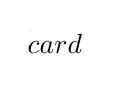
\begin{tikzpicture}[x=.006cm,y=-.006cm,baseline=(root-card-two-base.base)]
\path[use as bounding box] (0,0) rectangle (150,75);
\node[anchor=base west,inner sep=0pt,outer sep=0pt] (root-card-two-base) at (0,55) {$\operatorname{card}$};
\fill[gray!60] (5,6) ellipse (1.2 and 1.2);
\node[inner sep=0pt,outer sep=0pt] at (5,6) {$\unsure{\phantom{\cdot}}$};
\end{tikzpicture}}
